Proper modeling of \ww\ background distributions is critical for the
analysis. We use high \mll\ region to normalize \ww\ background in the
cut-based analysis and we rely on \mll\ and \mt\ distributions for the
2D fit. A number of generators were used to study how consistent
predictions are. We considered the following options:
\begin{itemize}
    \item {\bf Madgraph + Pythia6} - LO, up to two jets at matrix element level,
    full simulation and reconstruction. Only double-resonant
    contributions are included. Default sample in all CMS results in
    this channel.

    \item {\bf MC@NLO + Herwig6} - NLO, up to one jet at matrix element level,
    full simulation and reconstruction. Only double-resonant
    contributions are included. Used as an alternative. QCD scale
    variation samples are available as well.

    \item {\bf POWHEG + Pythia6} - NLO, up to one jet at matrix element level,
    full simulation and reconstruction. Includes both single and
    double resonant contributions. Available only for 8~\TeV{}.

    \item {\bf aMC@NLO} - NLO, up to one jet at matrix element level,
    generator level only. Includes both single and double resonant
    contributions.
\end{itemize}

Table~\ref{tab:appendix_wwshape_gen} shows the ratio of events in a
signal region for low mass Higgs with respect to full fit range used
in 2D fit for two observables \mll\ and \mt\ at generator
level. Figure~\ref{fig:appendix_wwshape_mcatnlo} and
Figure~\ref{fig:appendix_wwshape_ref} show corresponding
distributions.

While the generator level tests allow for a quick check of a number of
options, the ultimate comparison comes from fully simulated and
reconstructed samples. Table~\ref{tab:appendix_wwshape_hww} shows the
ratio of events in a signal region for low mass Higgs with respect to
full fit range used in 2D fit for two observables \mll\ and \mt\ at
generator level. Events are required to pass the following selections:
\begin{itemize}
   \item zero-jet requirement
   \item full lepton selection
   \item \emu\ and \mue\ channels only 
   \item top and extra-lepton veto
   \item minMET $>20$~\GeV\
   \item dilepton $\pt>30$~\GeV\
   \item $\mt>60$~\GeV\
\end{itemize}
Figure~\ref{fig:appendix_wwshape_mcatnlo_hww} and
Figure~\ref{fig:appendix_wwshape_ref_hww} show corresponding
distributions. As one can see our choice of central shape (Madgraph)
and alternative generator (MC@NLO) plus the QCD scale variation covers
a full spectrum of possibilities. All the shapes are quite similar and
with a large enough dataset 2D fit should have no issue to find a
shape that best fits data in regions dominated by \ww{}.

\begin{table}
\begin{center}
\begin{tabular}{ p{6cm} | c | c }
\hline
       Monte Carlo sample & $\frac{\mll\in[12,48]}{\mll\in[12,200]}$ & $\frac{\mt\in[60,125]}{\mt\in[60,280]}$ \\
\hline
       Madgraph          & $22.89\pm0.26$ \% & $70.16\pm0.53$ \%\\
       MC@NLO            & $23.61\pm0.33$ \% & $75.63\pm0.71$ \%\\
       MC@NLO scale up   & $23.69\pm0.34$ \% & $76.54\pm0.71$ \%\\
       MC@NLO scale down & $23.89\pm0.34$ \% & $75.49\pm0.70$ \%\\
       POWHEG            & $23.81\pm0.25$ \% & $74.22\pm0.52$ \%\\
       aMC@NLO           & $24.43\pm0.24$ \% & $74.52\pm0.48$ \%\\
\hline
\end{tabular}
\caption{Ratio of events in a signal region for
low mass Higgs with respect to full fit range used in 2D fit for two
observables \mll\ and \mt\ at generator level}
\label{tab:appendix_wwshape_gen}
\end{center}
\end{table}

\begin{table}
\begin{center}
\begin{tabular}{ p{6cm} | c | c }
\hline
       Monte Carlo sample & $\frac{\mll\in[12,48]}{\mll\in[12,200]}$ & $\frac{\mt\in[60,125]}{\mt\in[60,280]}$ \\
\hline
       Madgraph          & $26.08\pm0.21$ \% & $70.46\pm0.33$ \%\\
       MC@NLO            & $26.43\pm0.38$ \% & $72.02\pm0.61$ \%\\
       MC@NLO scale up   & $27.08\pm0.38$ \% & $72.81\pm0.60$ \%\\
       MC@NLO scale down & $25.91\pm0.38$ \% & $71.17\pm0.61$ \%\\
       POWHEG            & $26.48\pm0.28$ \% & $71.17\pm0.44$ \%\\
\hline
\end{tabular}
\caption{Ratio of events in a signal region for
low mass Higgs with respect to full fit range used in 2D fit for two
observables \mll\ and \mt\ at the Higgs event selection level.}
\label{tab:appendix_wwshape_hww}
\end{center}
\end{table}

\begin{figure}[!hbtp]
\centering
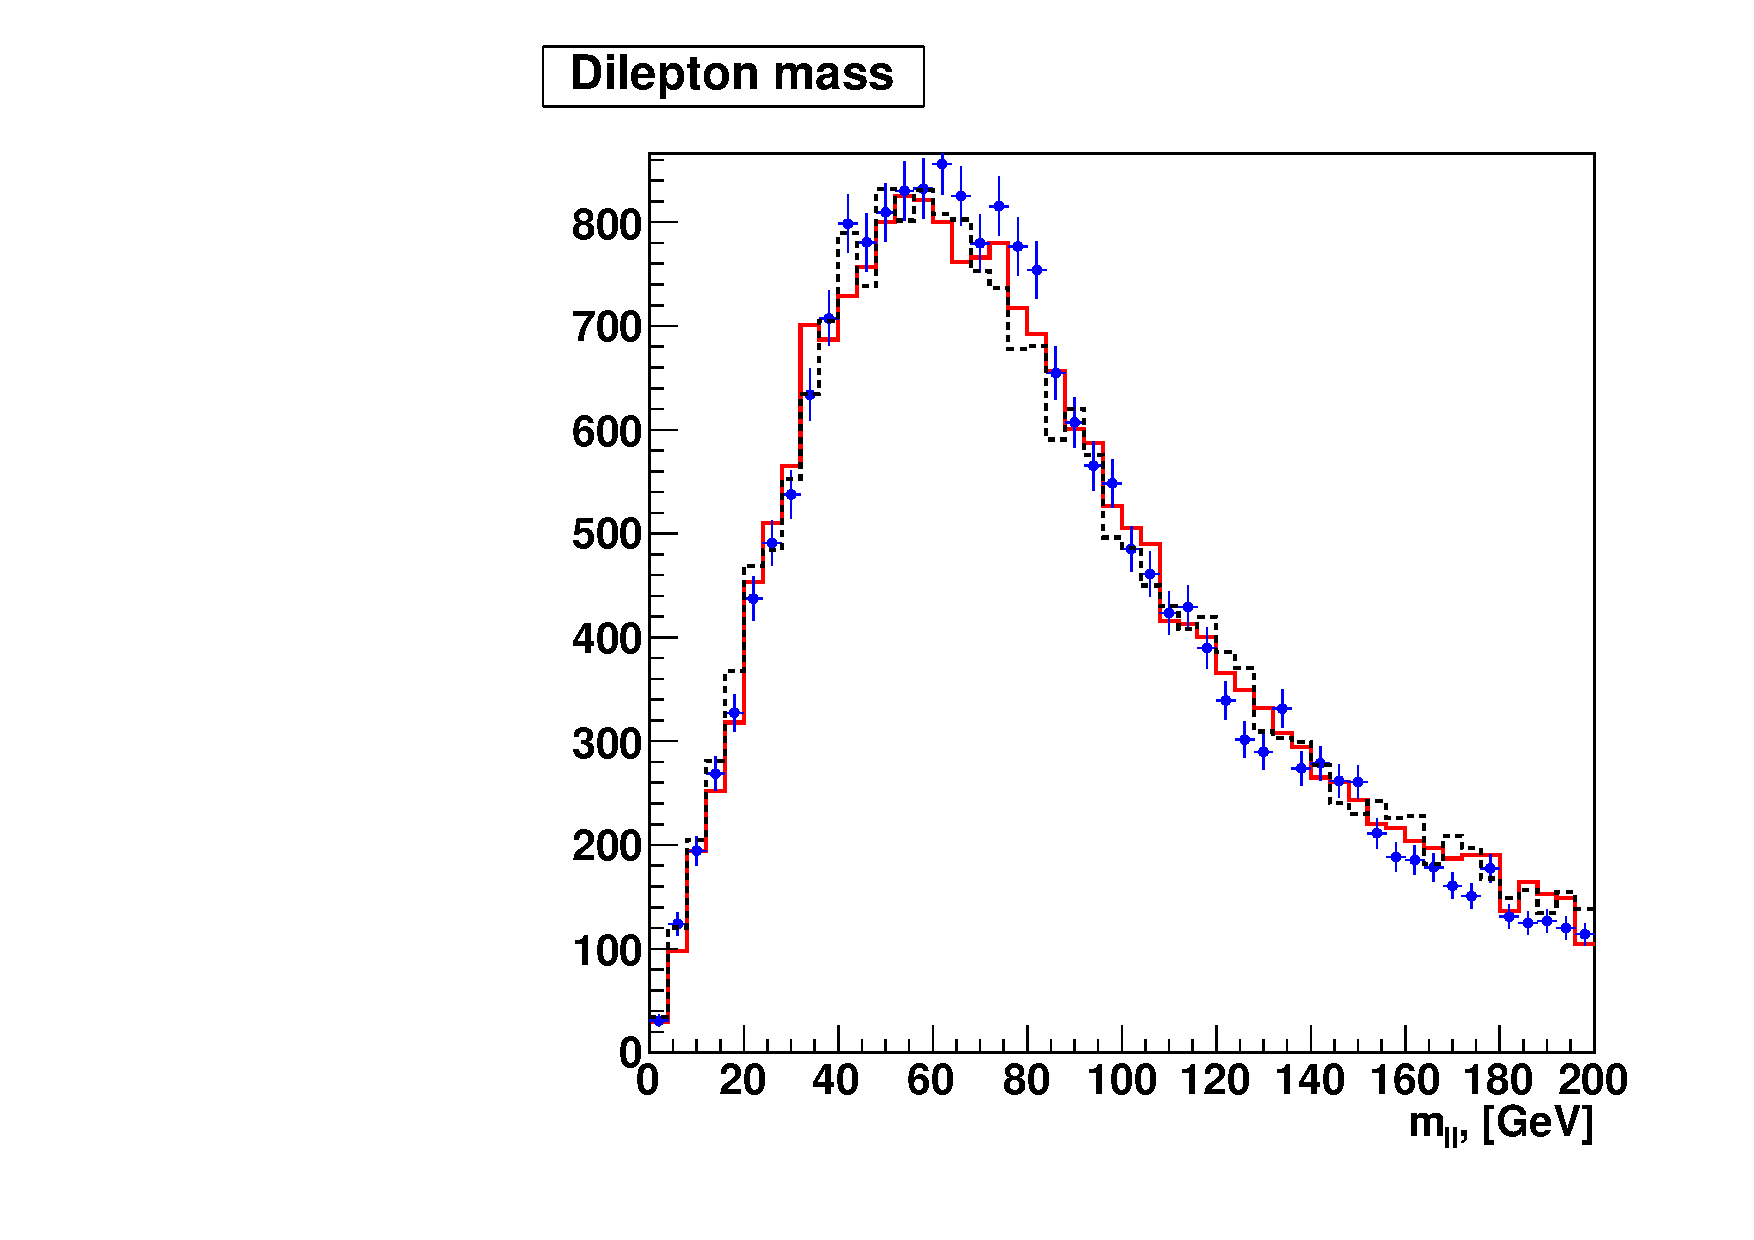
\includegraphics[width=.45\textwidth]{figures/wwshape_mcatnlo_mll}
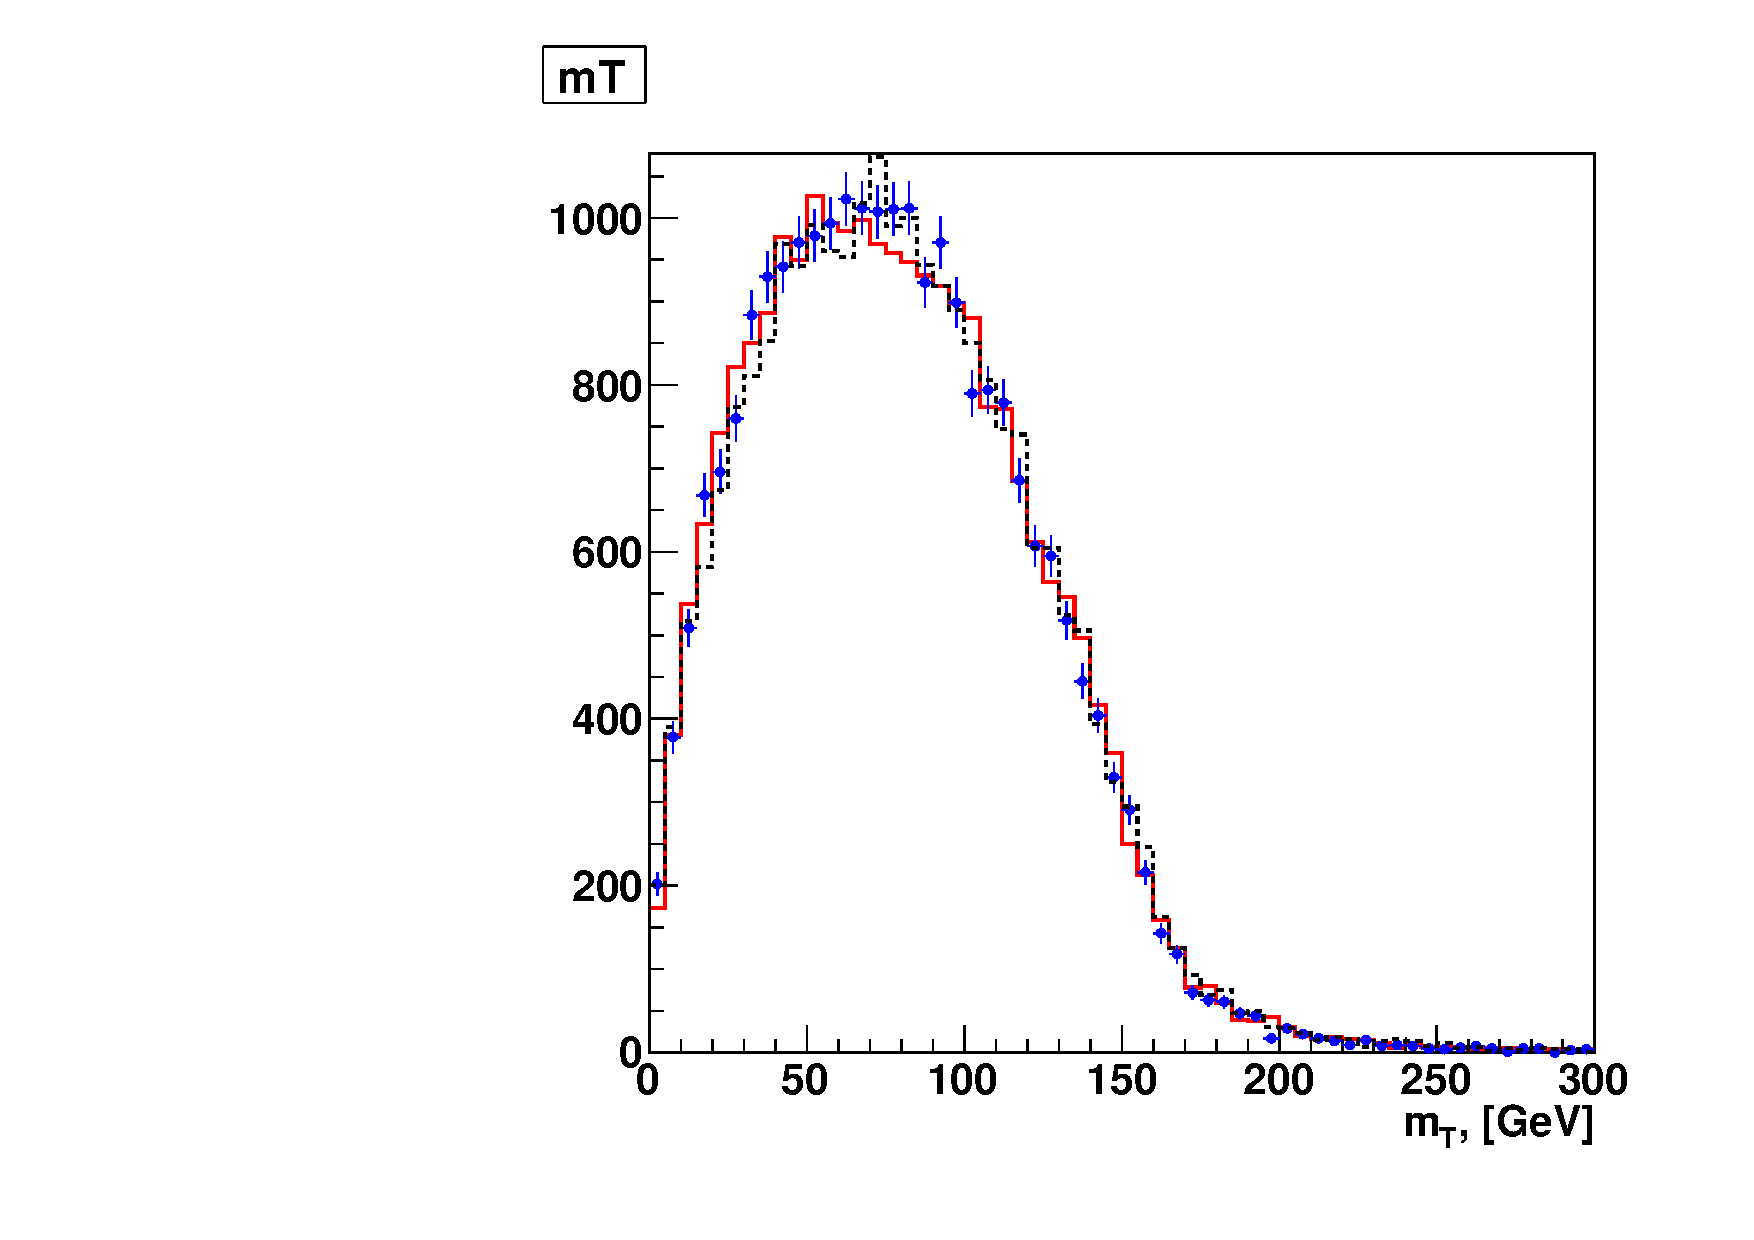
\includegraphics[width=.45\textwidth]{figures/wwshape_mcatnlo_mt}
\caption{MC@NLO generator level distributions (red solid line - central shape, blue points - qcd scale up, black dashed line - qcd scale down}
\label{fig:appendix_wwshape_mcatnlo}
\end{figure}

\begin{figure}[!hbtp]
\centering
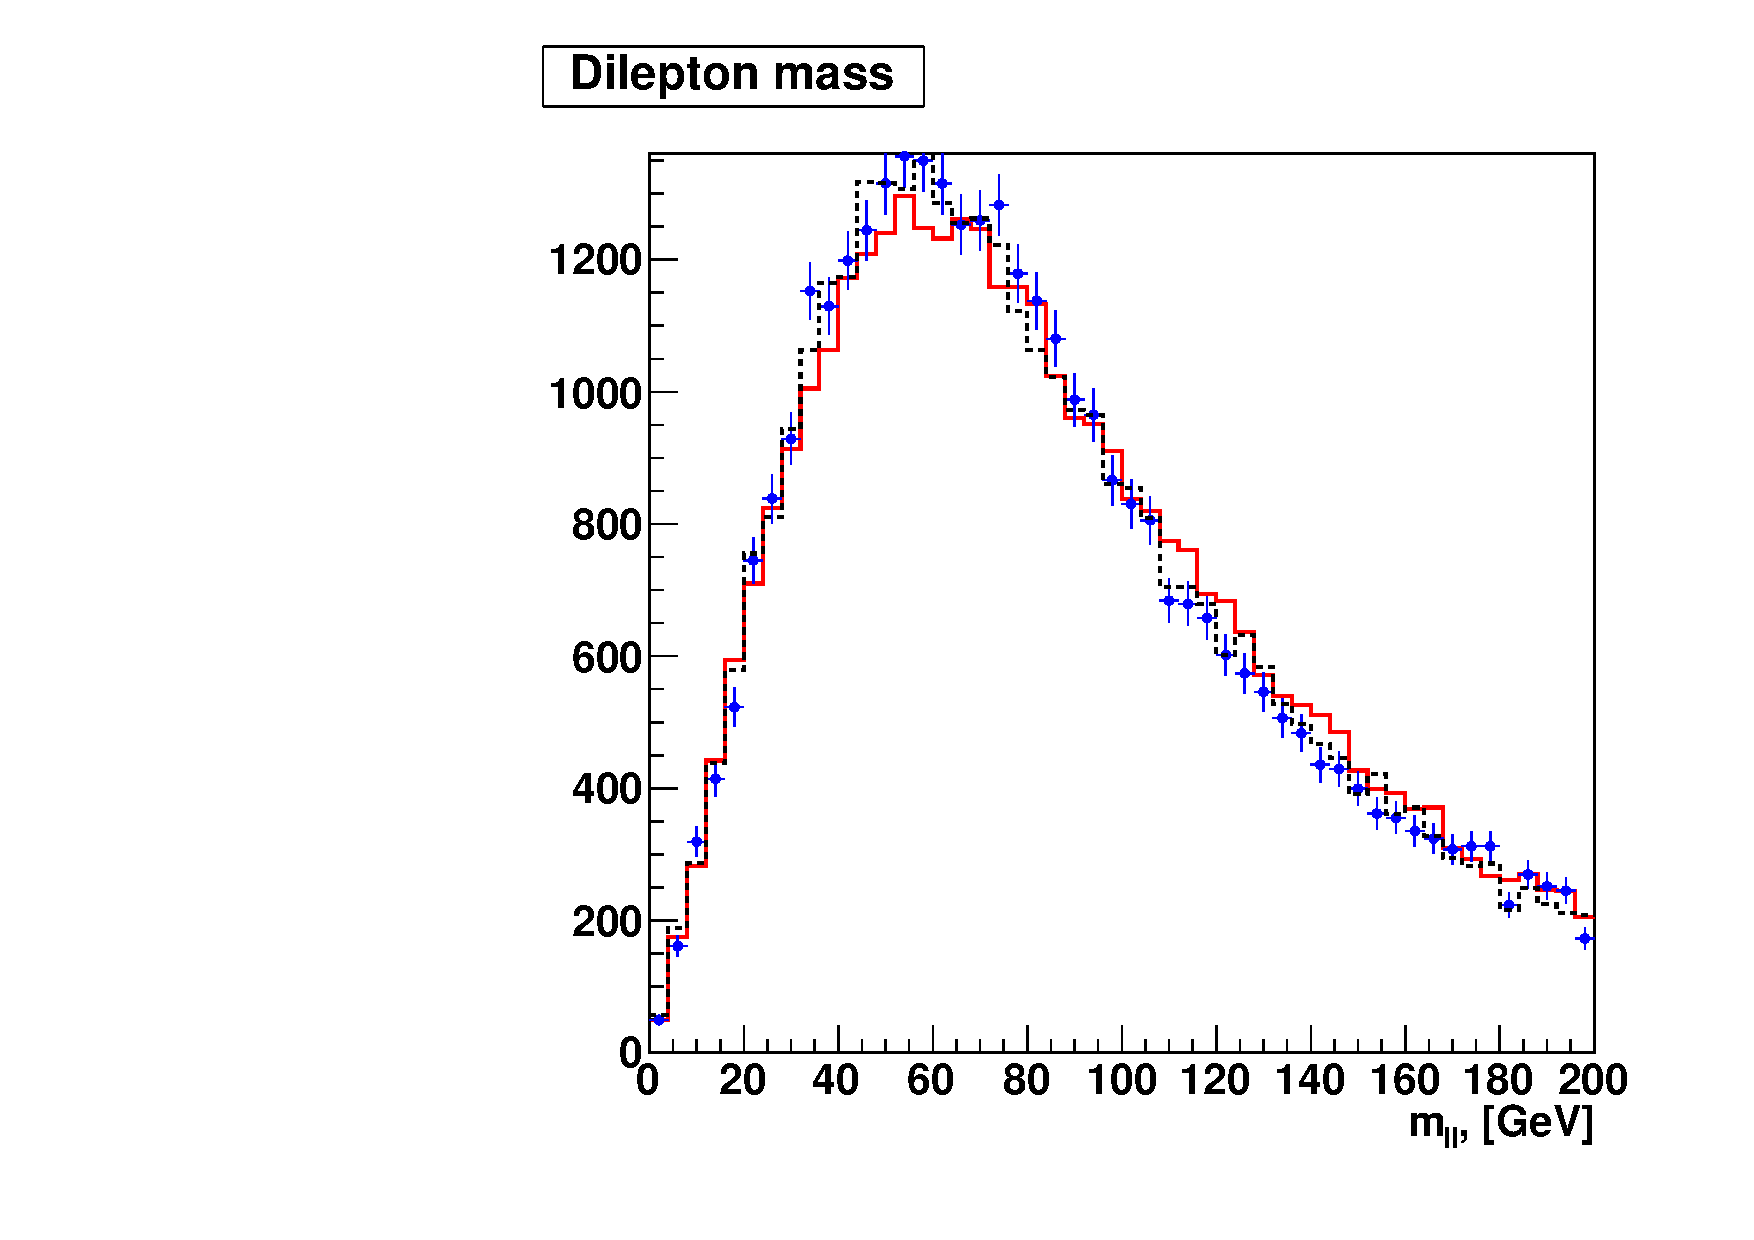
\includegraphics[width=.45\textwidth]{figures/wwshape_ref_mll}
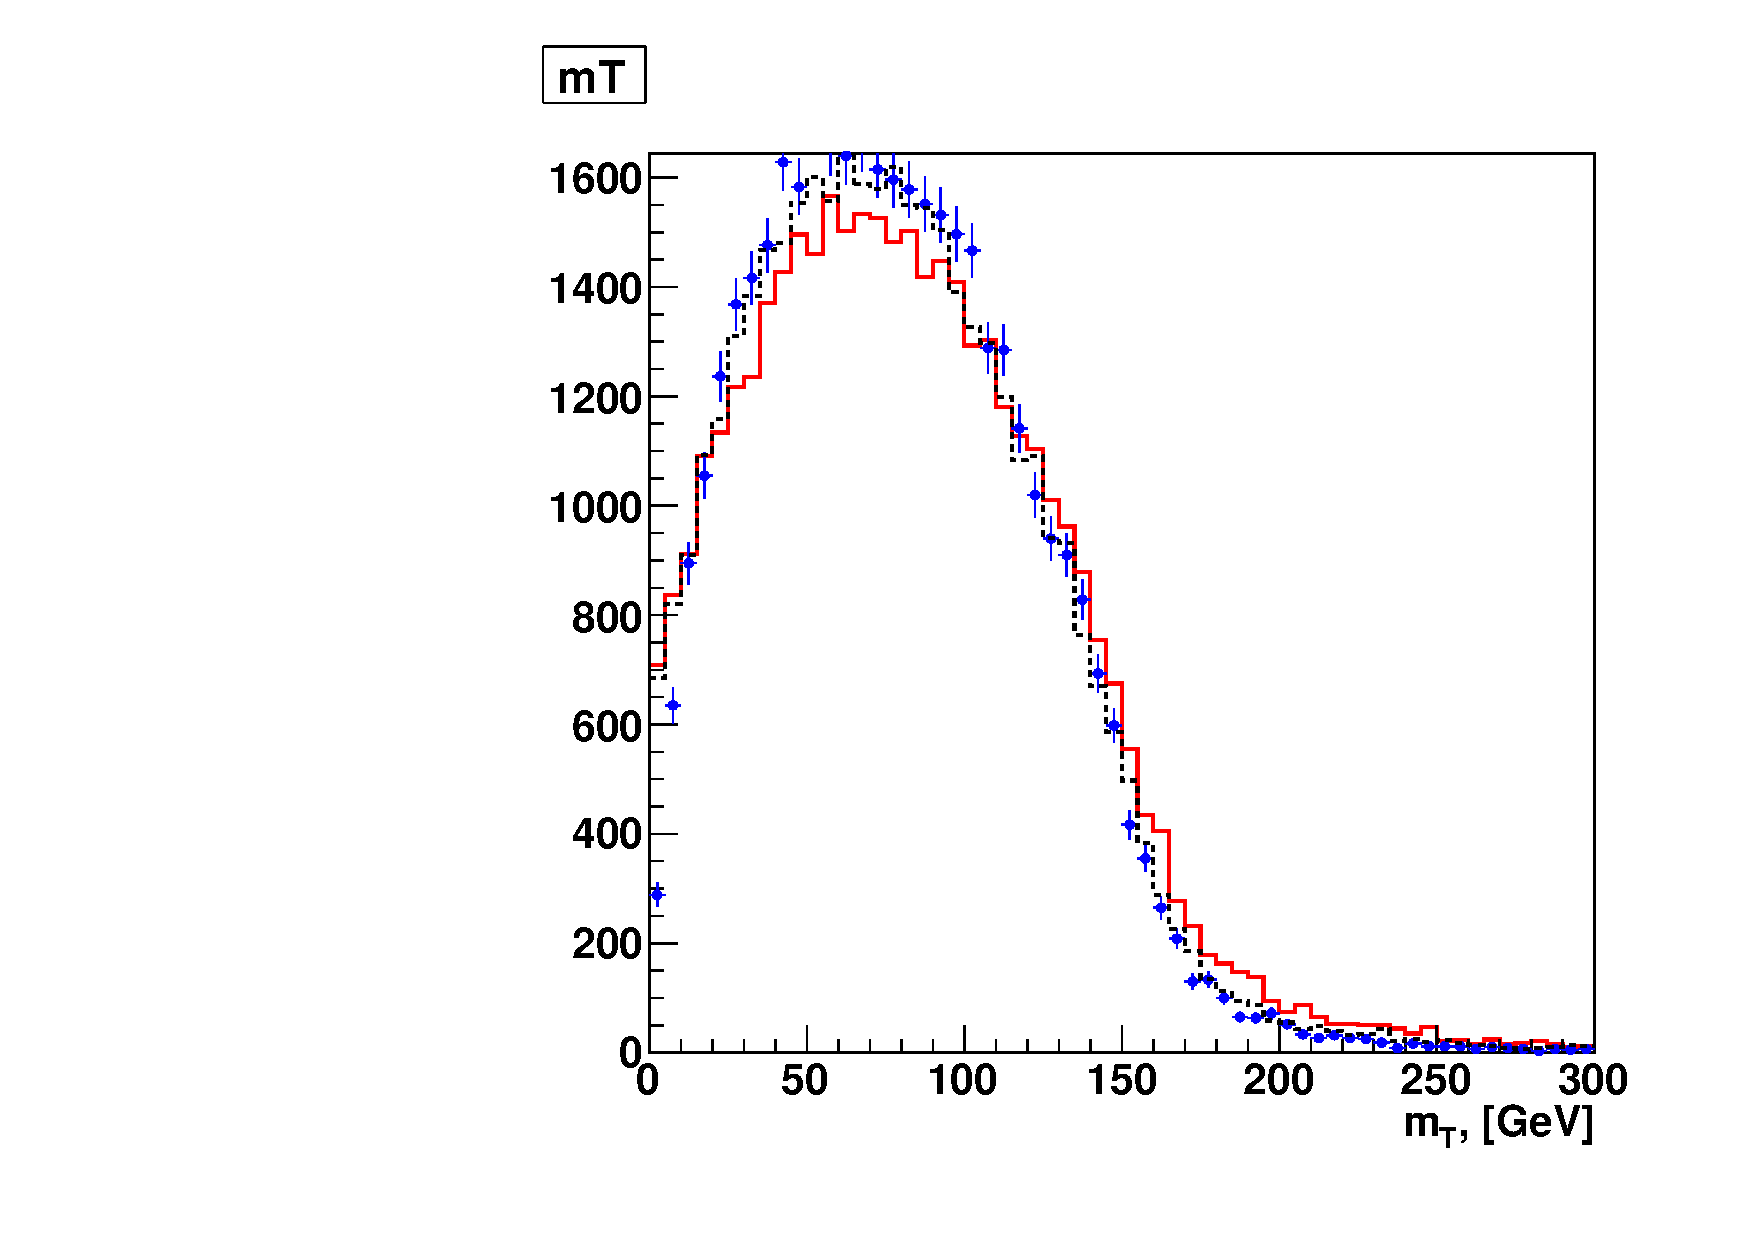
\includegraphics[width=.45\textwidth]{figures/wwshape_ref_mt}
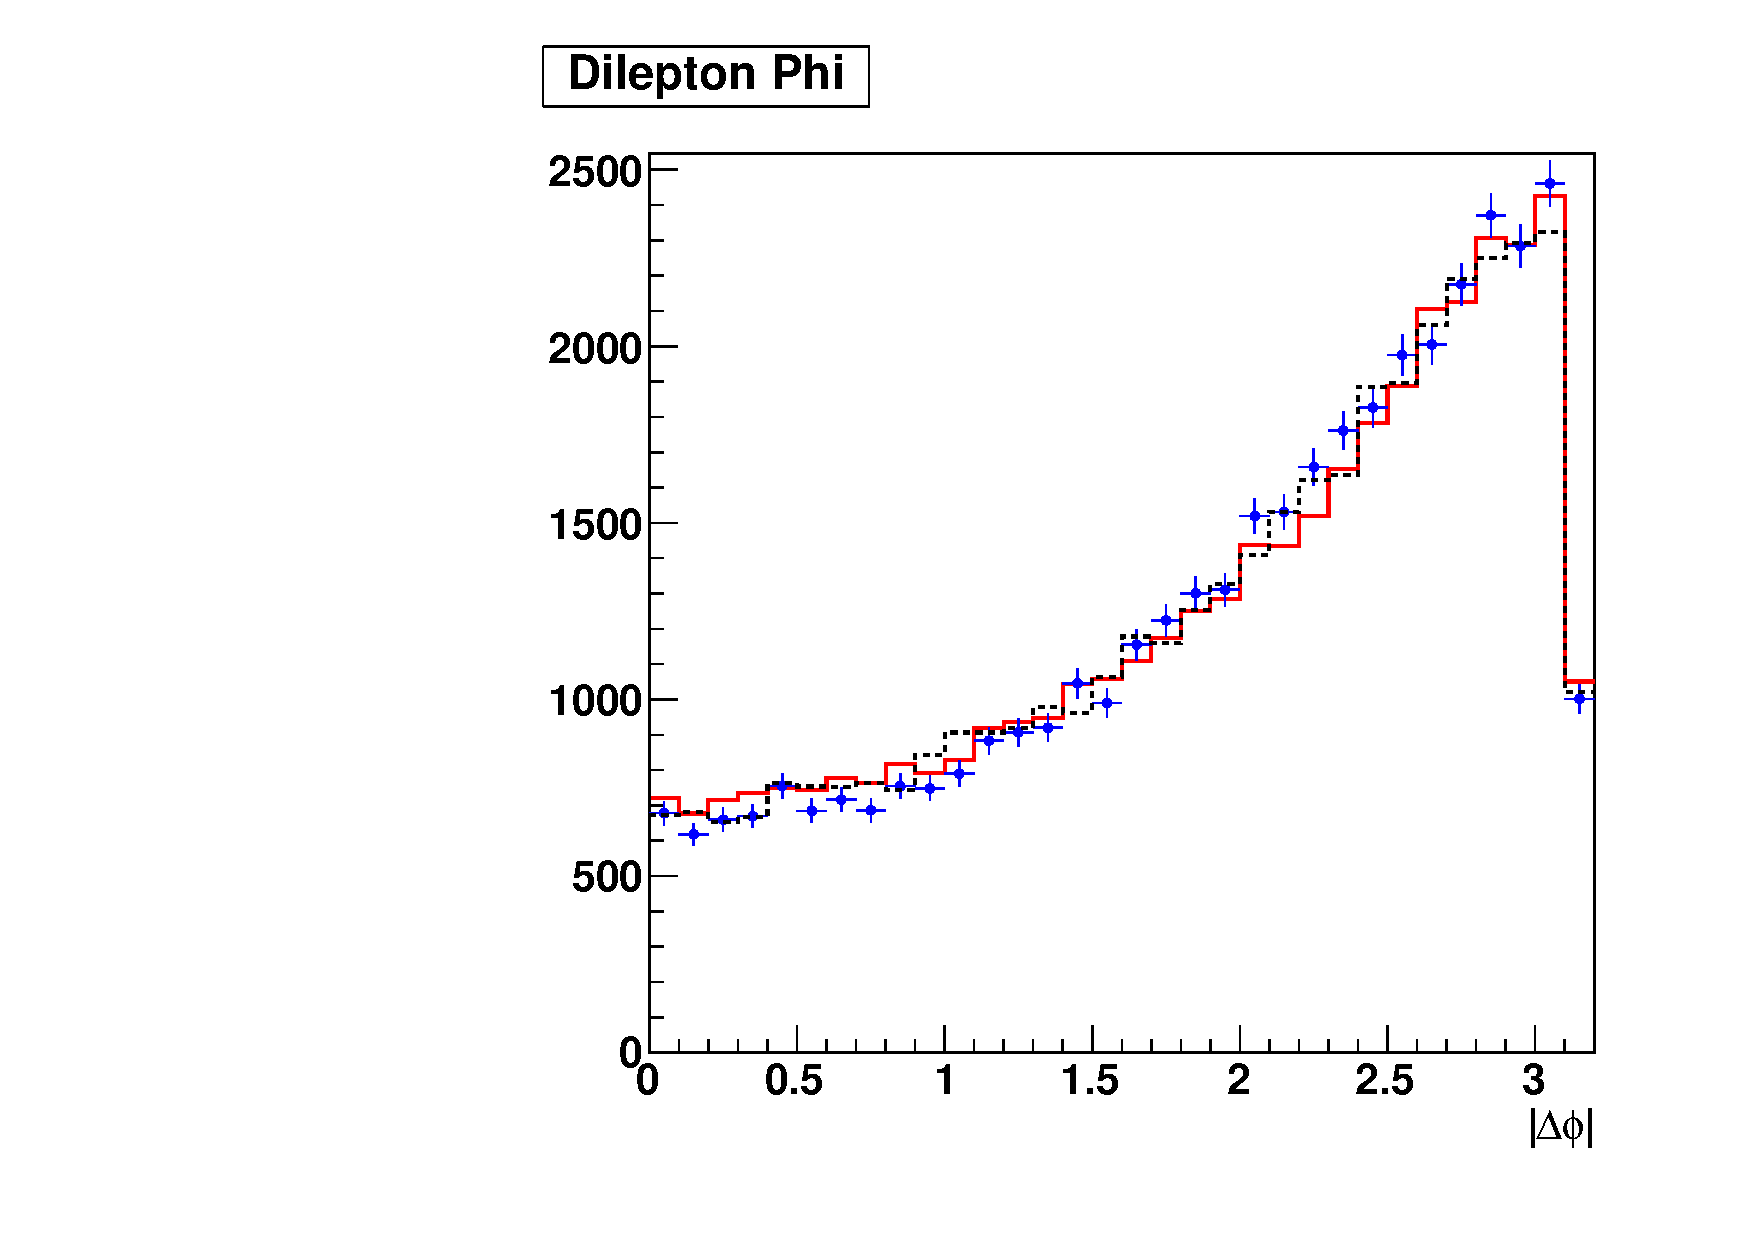
\includegraphics[width=.45\textwidth]{figures/wwshape_ref_dphi}
\caption{Generator level distributions for main samples (red solid line - Madgraph, blue points - MC@NLO, black dashed line - POWHEG}
\label{fig:appendix_wwshape_ref}
\end{figure}

\begin{figure}[!hbtp]
\centering
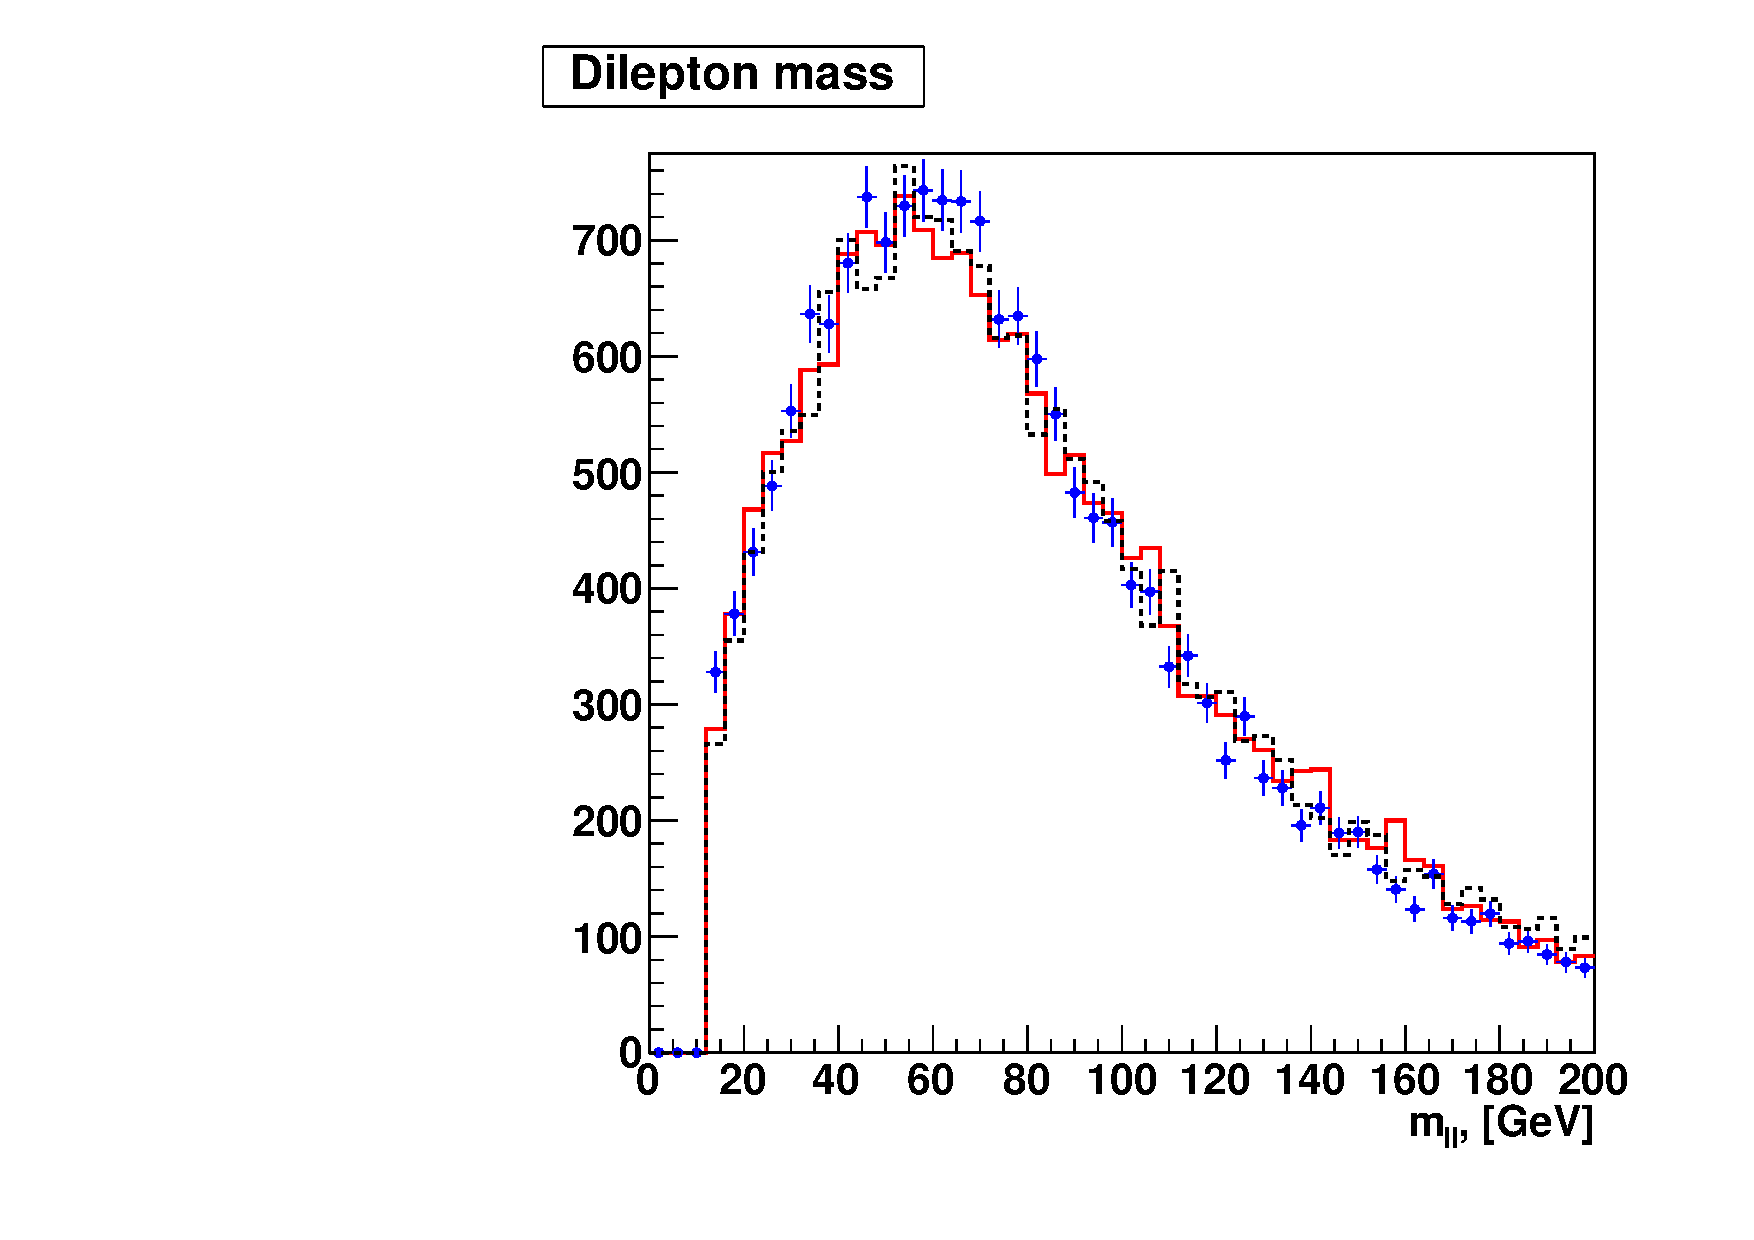
\includegraphics[width=.45\textwidth]{figures/wwshape_mcatnlo_mll_hww}
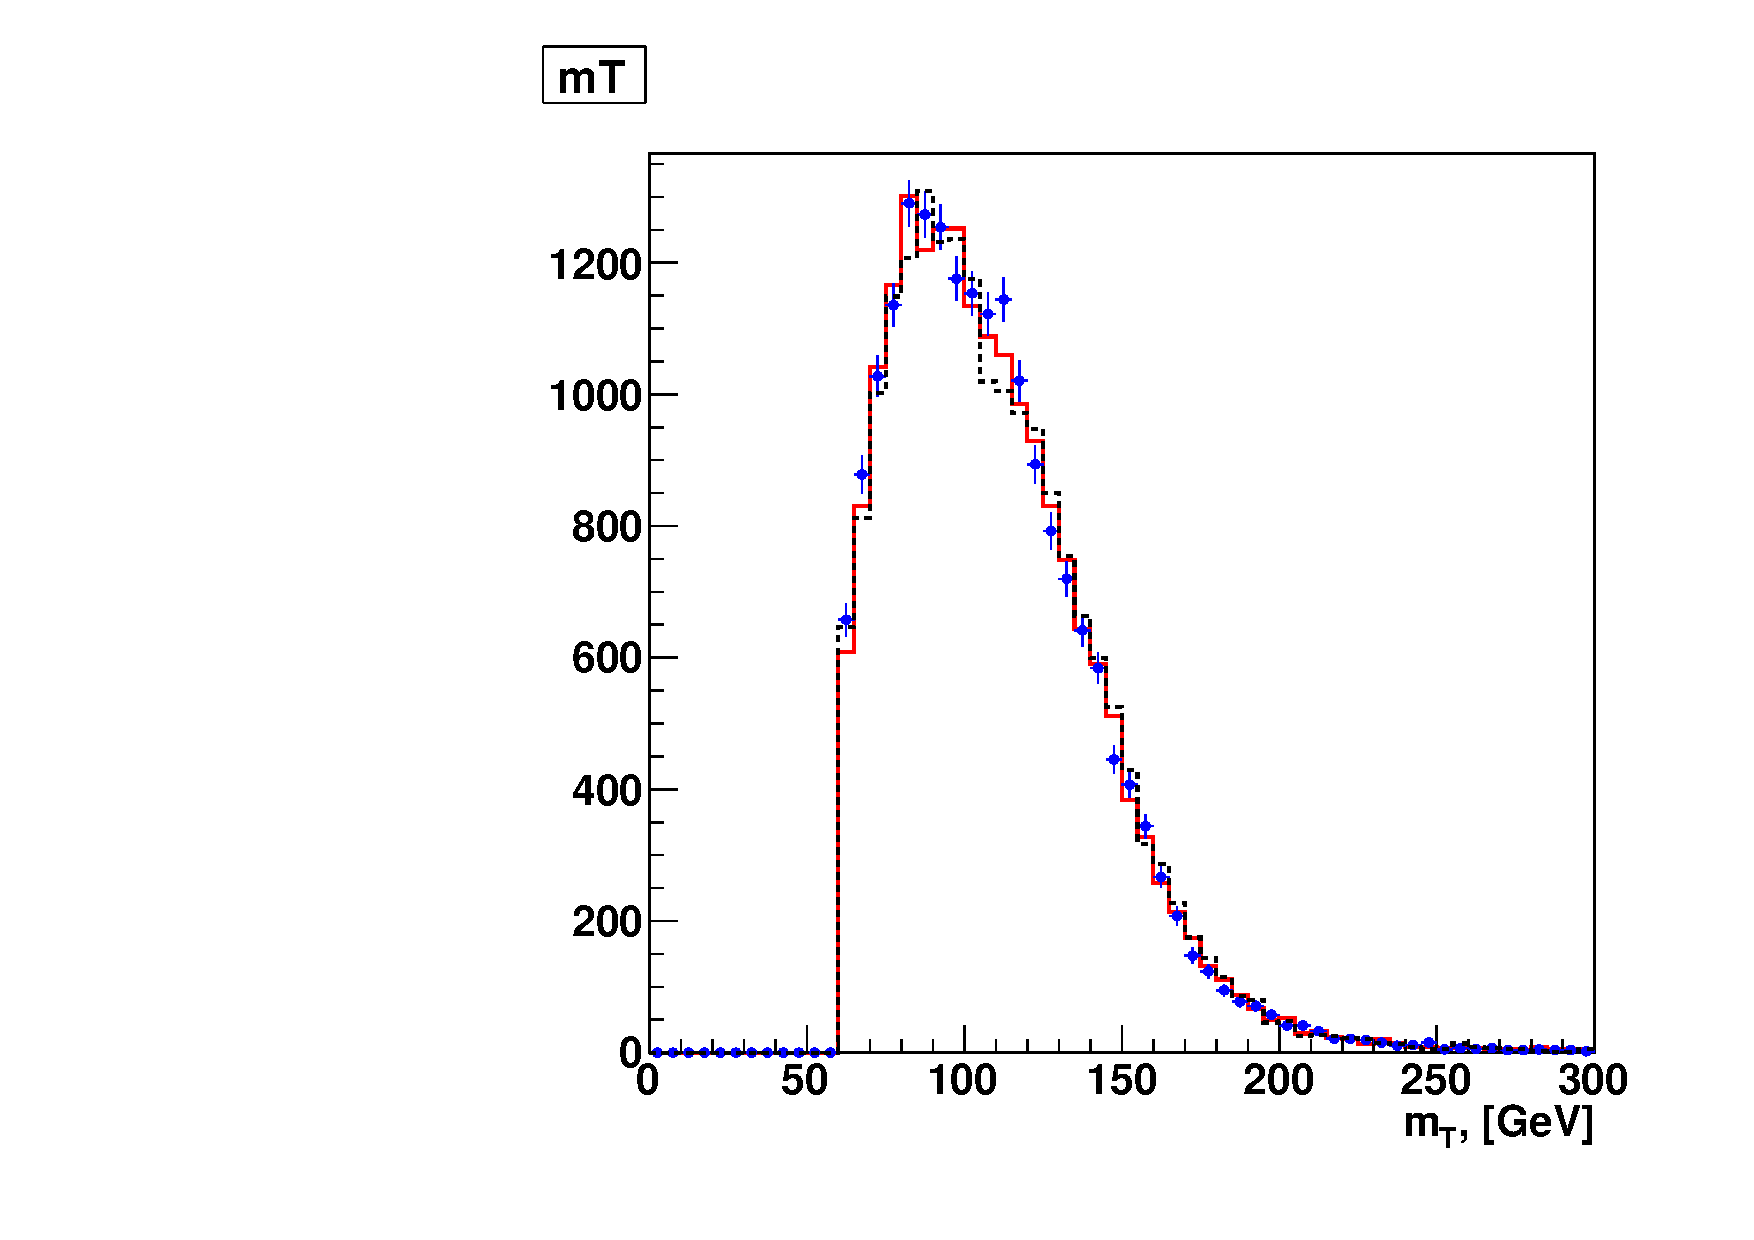
\includegraphics[width=.45\textwidth]{figures/wwshape_mcatnlo_mt_hww}
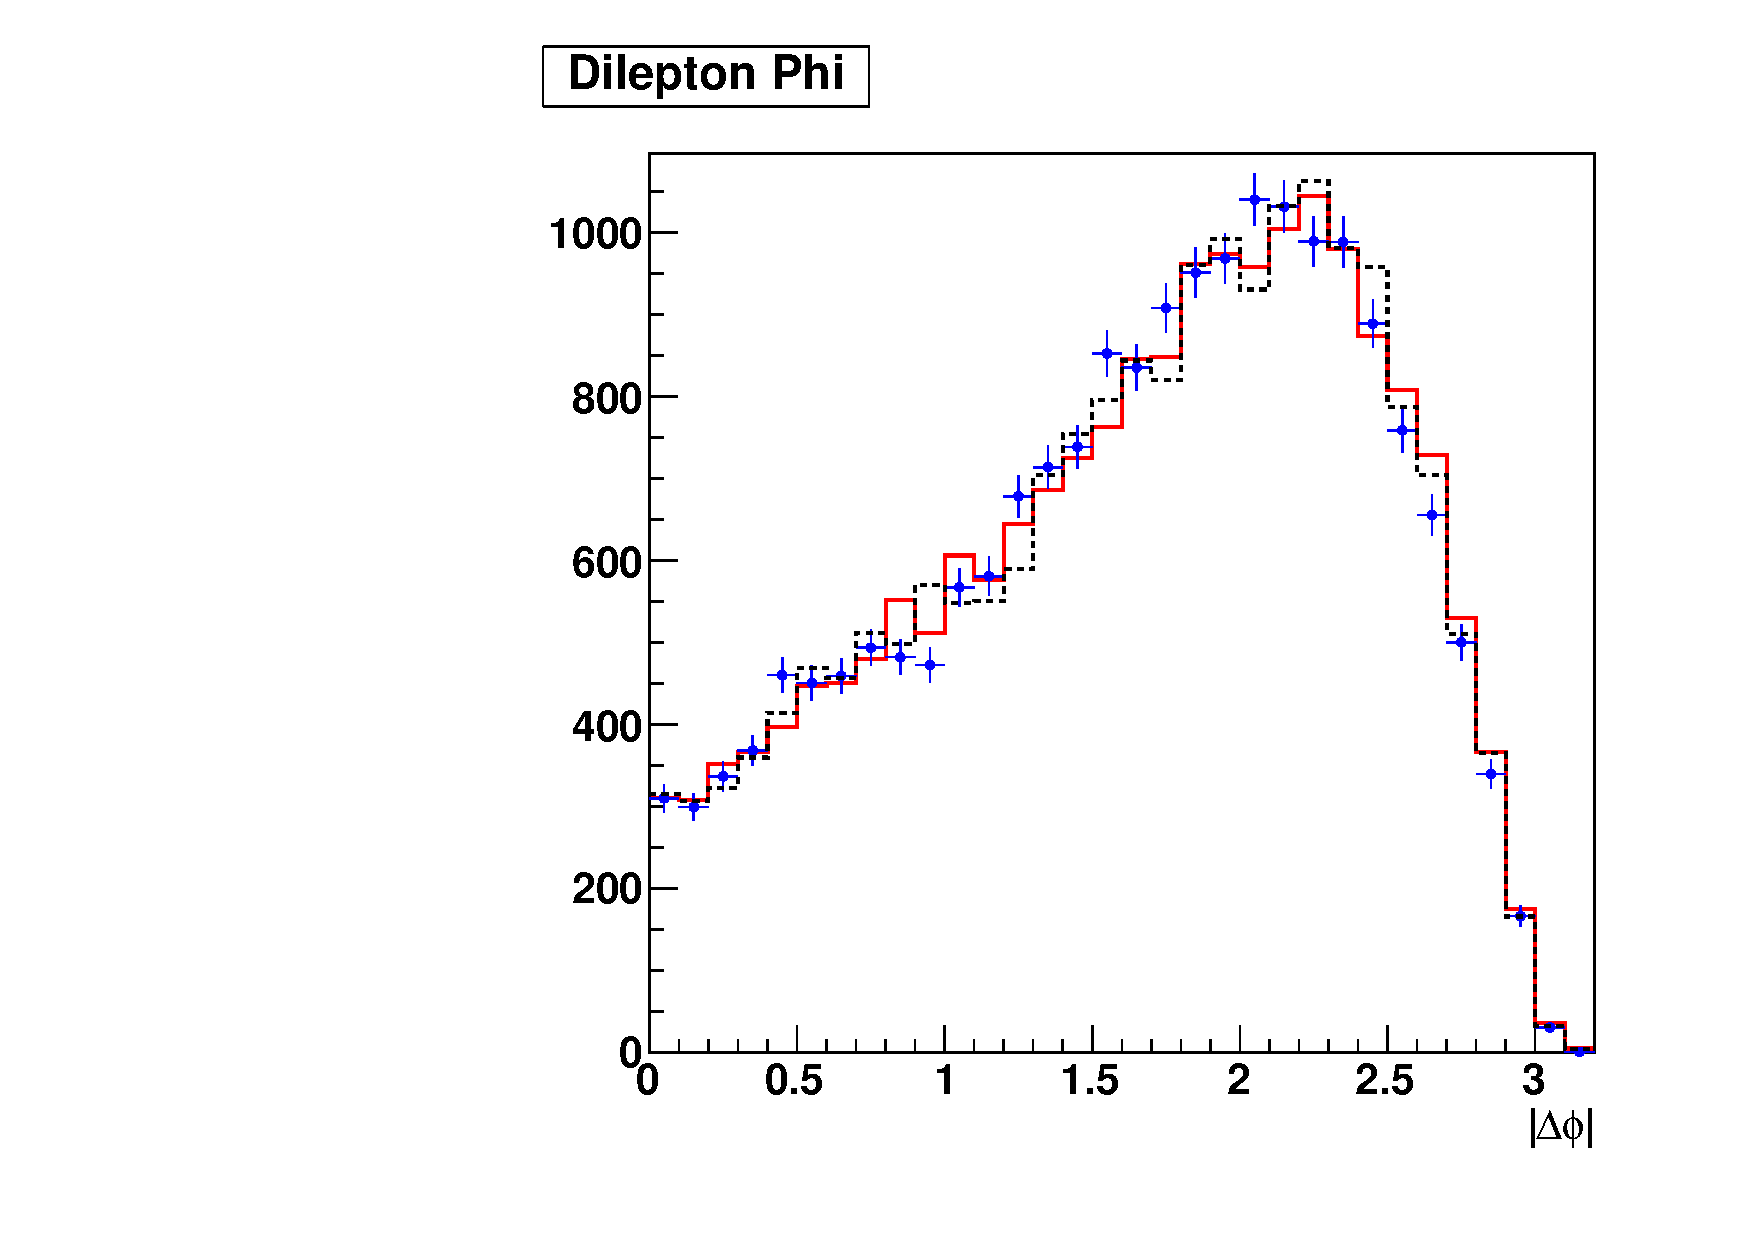
\includegraphics[width=.45\textwidth]{figures/wwshape_mcatnlo_dphi_hww}
\caption{MC@NLO distributions at the Higgs event selection level (red solid line - central shape, blue points - qcd scale up, black dashed line - qcd scale down}
\label{fig:appendix_wwshape_mcatnlo_hww}
\end{figure}

\begin{figure}[!hbtp]
\centering
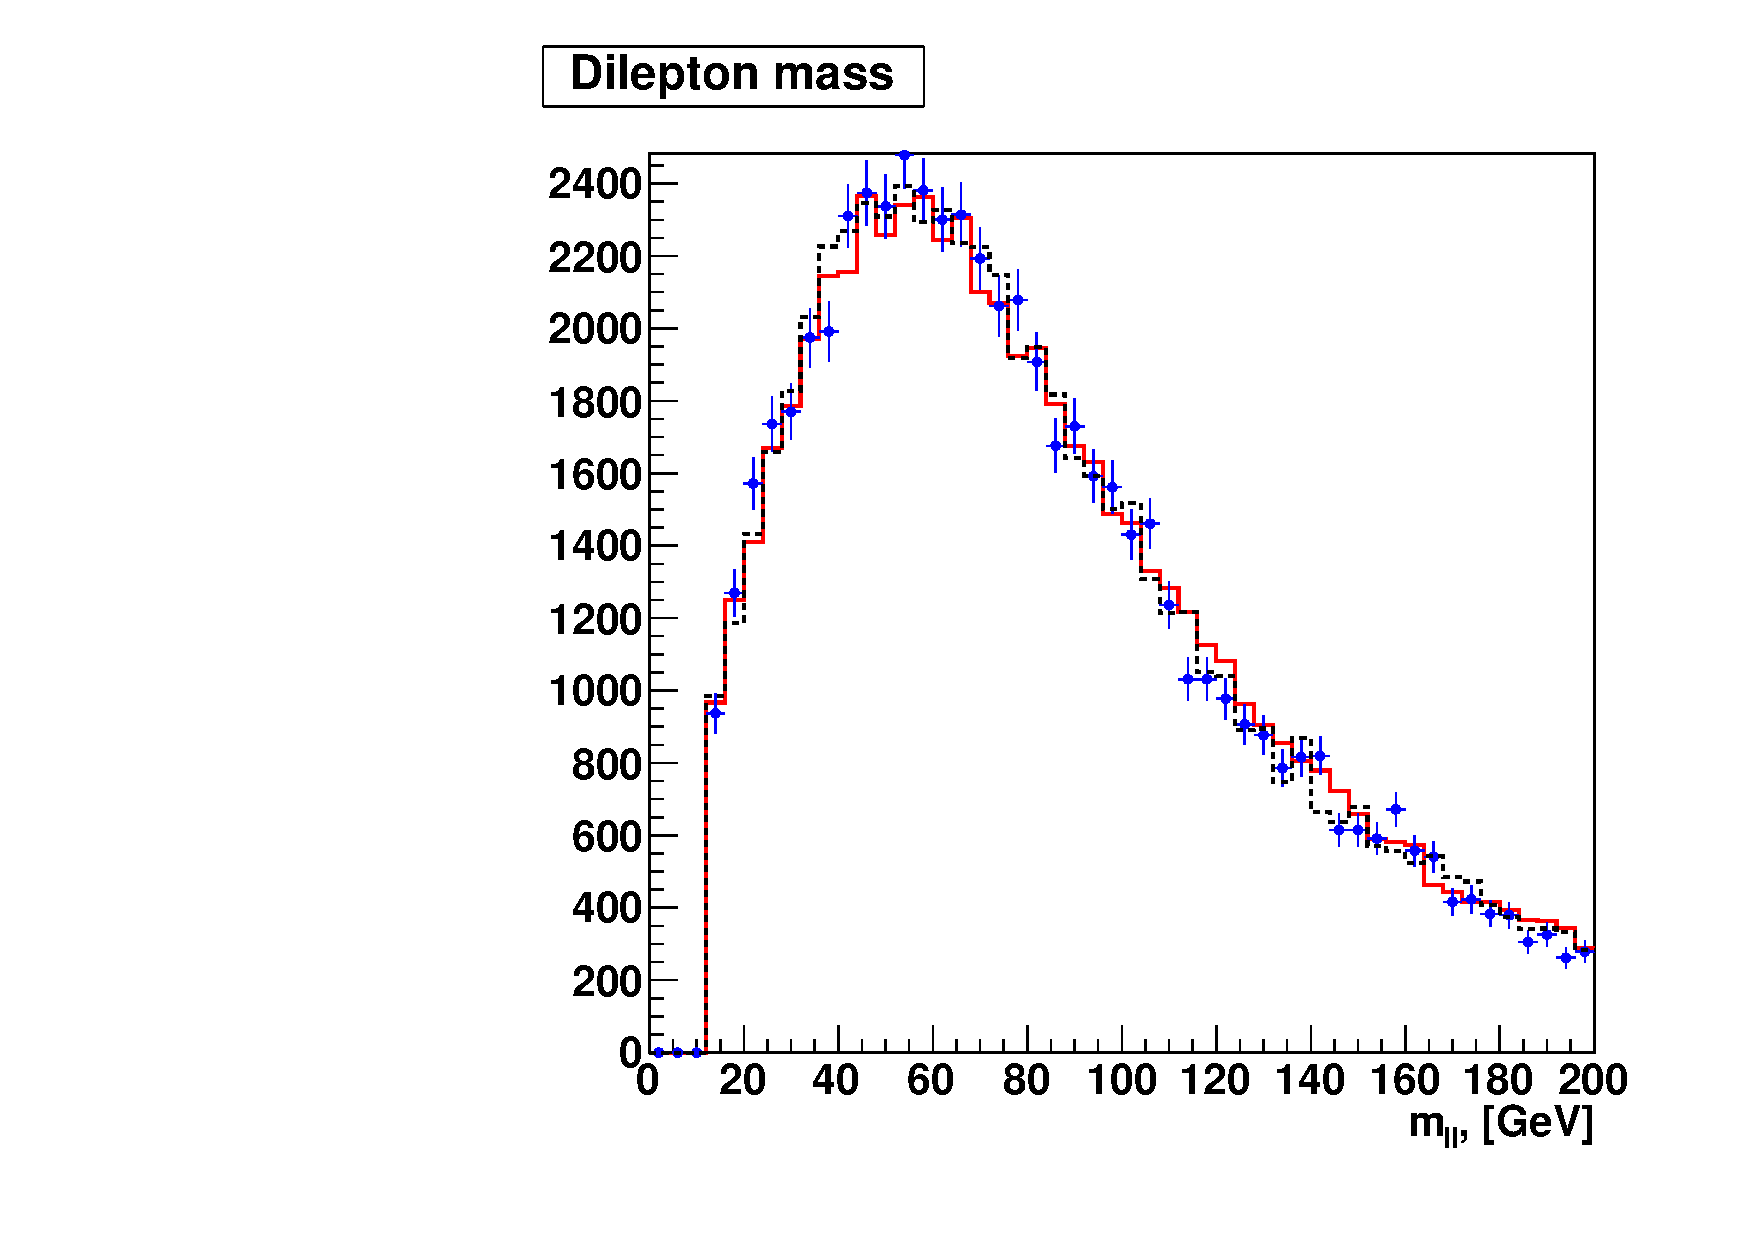
\includegraphics[width=.45\textwidth]{figures/wwshape_ref_mll_hww}
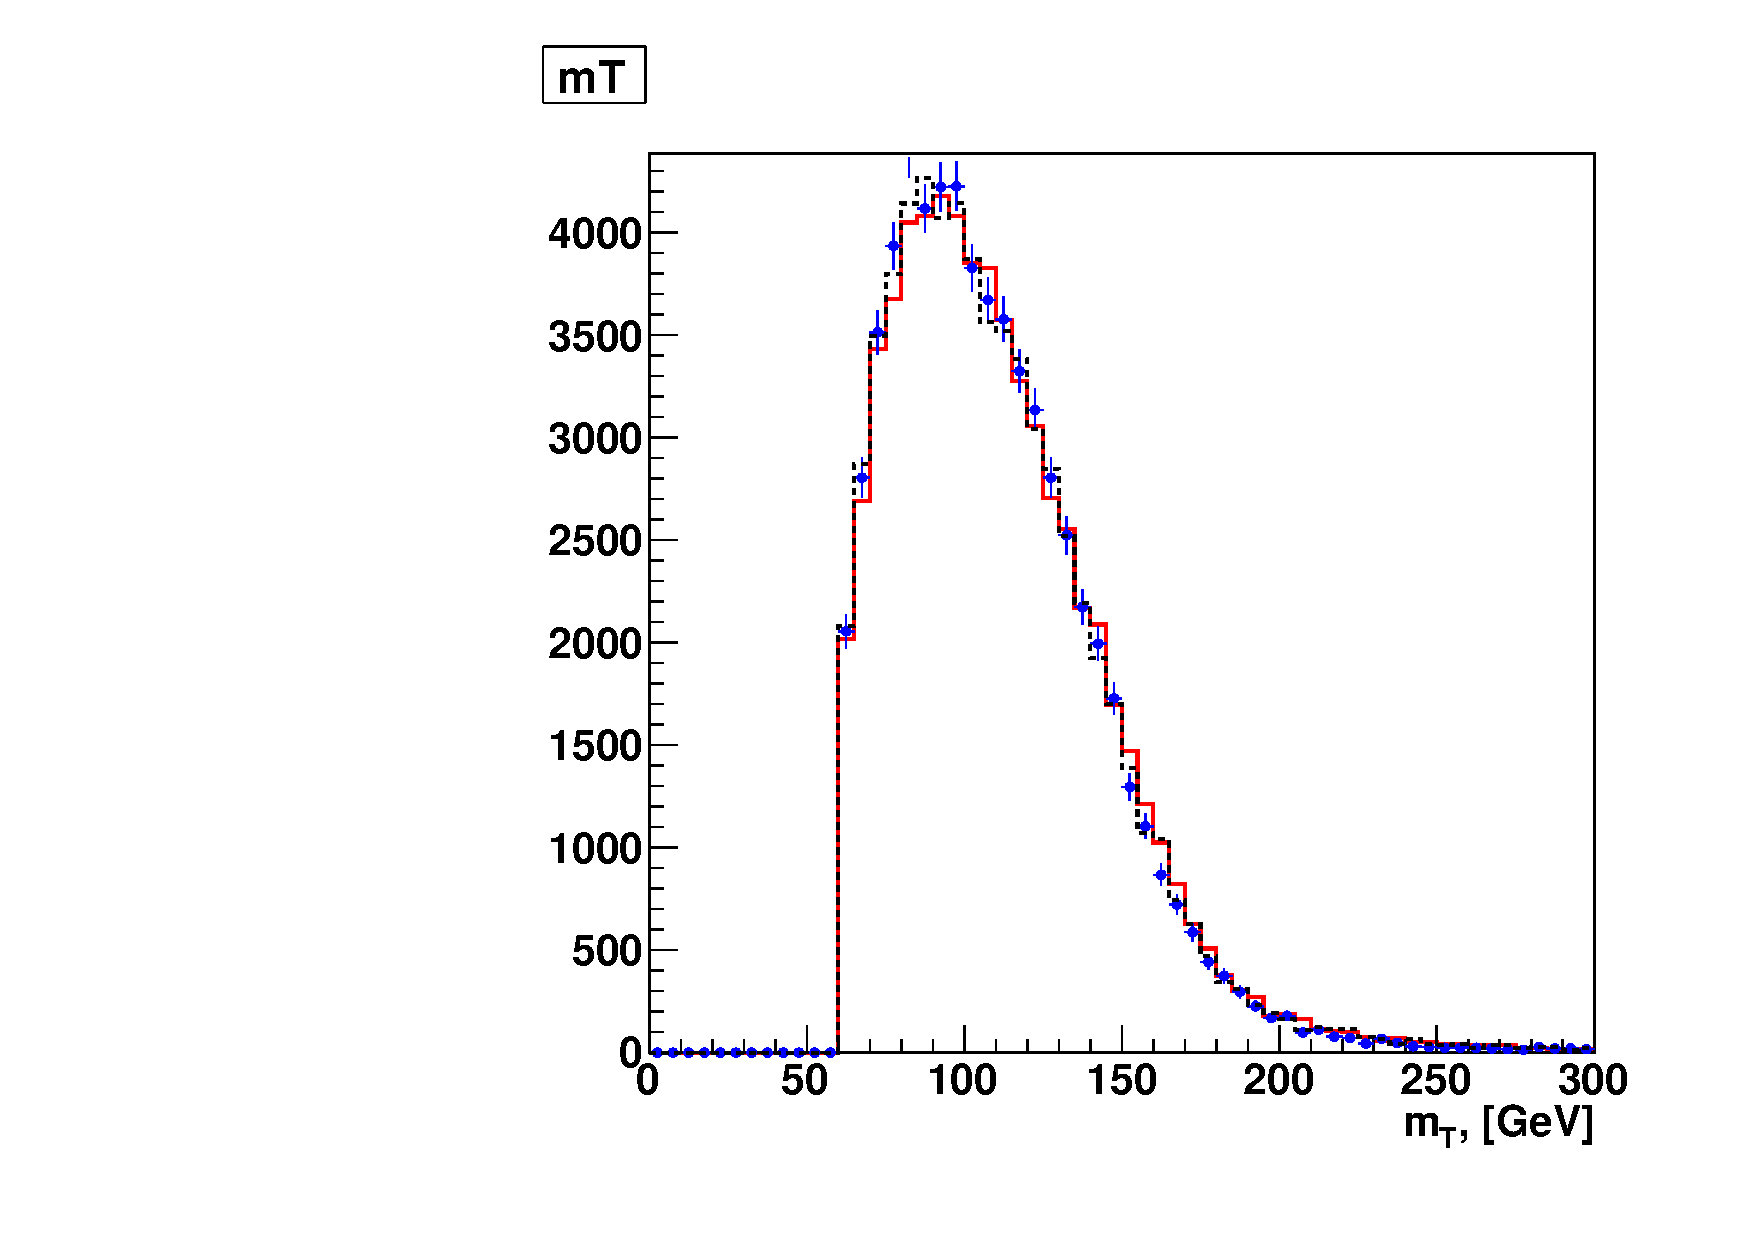
\includegraphics[width=.45\textwidth]{figures/wwshape_ref_mt_hww}
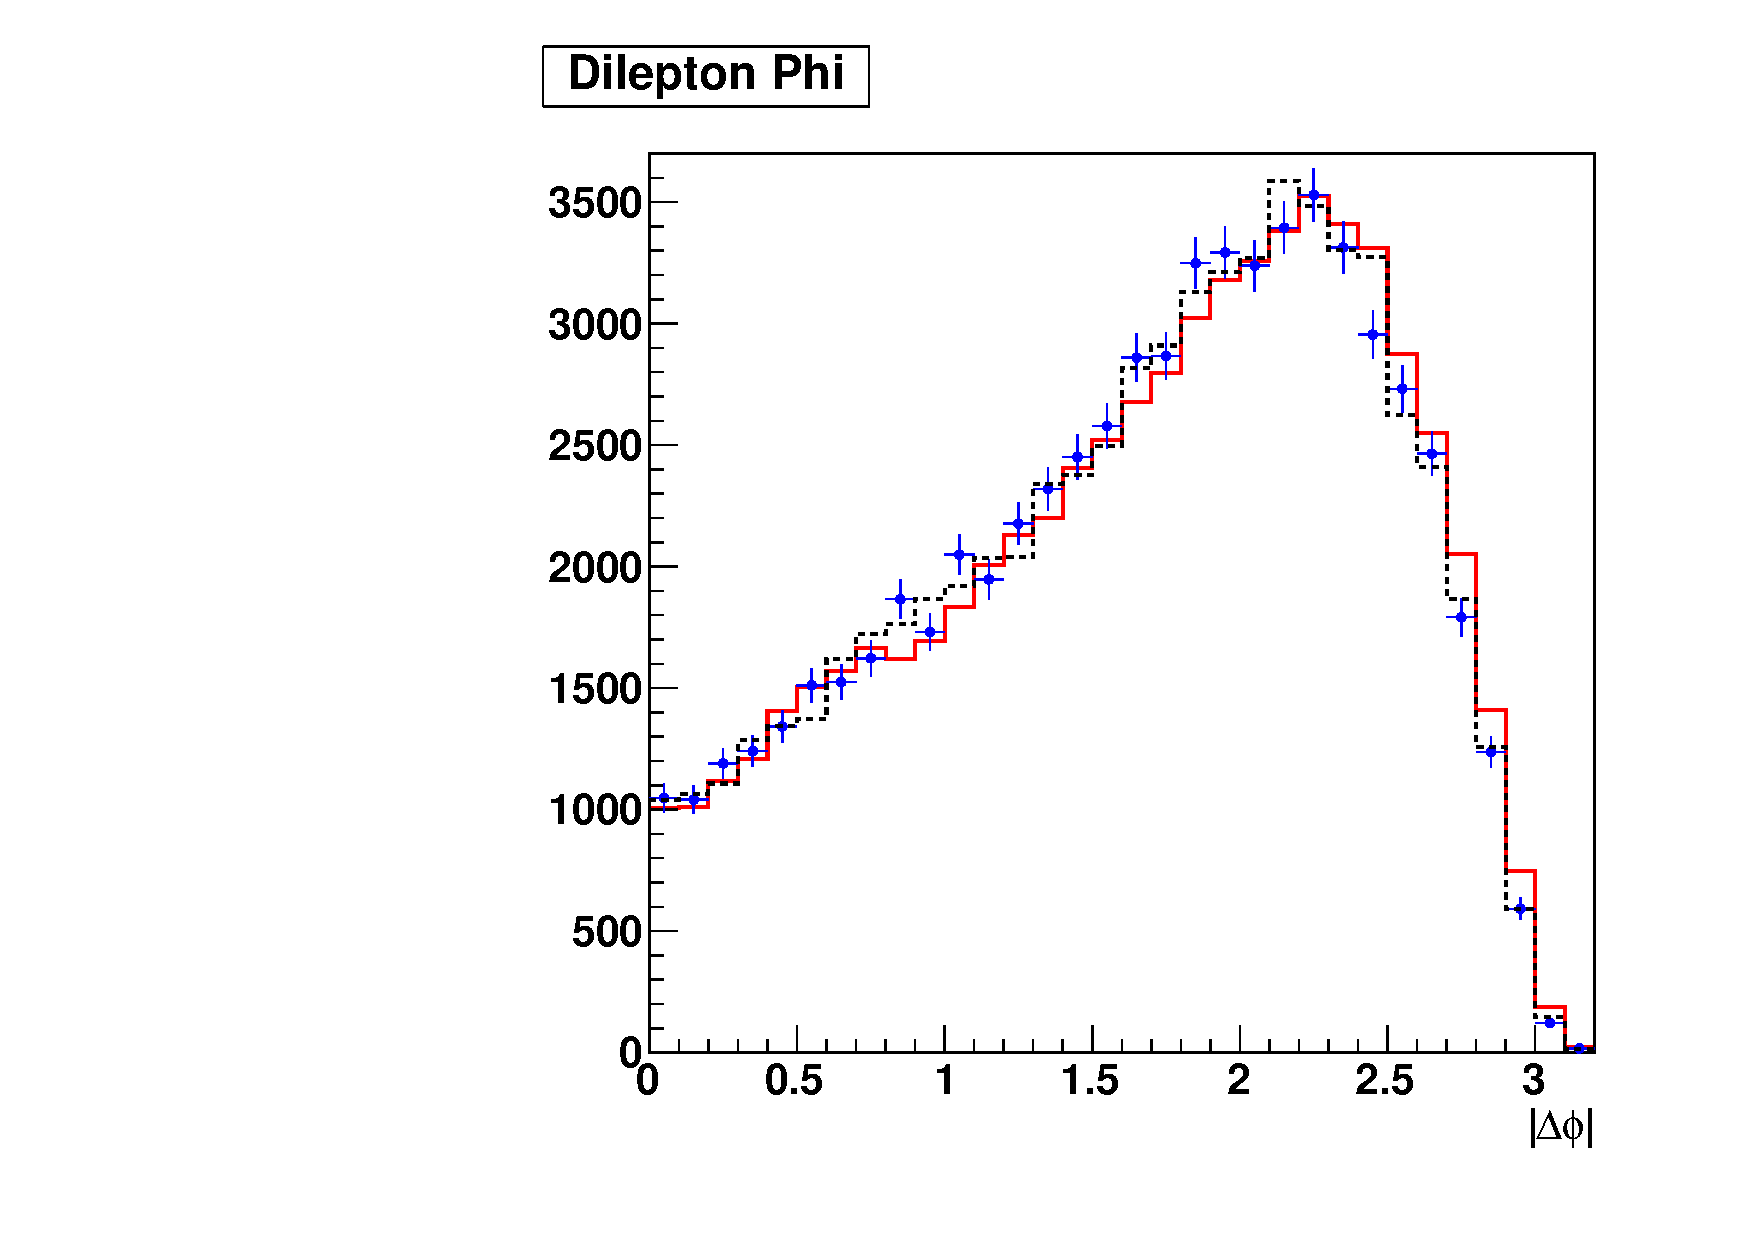
\includegraphics[width=.45\textwidth]{figures/wwshape_ref_dphi_hww}
\caption{Distributions at the Higgs event selection levels (red solid line - Madgraph, blue points - MC@NLO, black dashed line - POWHEG}
\label{fig:appendix_wwshape_ref_hww}
\end{figure}
